\chapter{Impact of Function-Call Tracing in the npm Ecosystem}
\label{sec:impact_study}

For the previous studies I have hand-picked the projects for the study, reason why for this study, first I wanted to perform an analysis on a larger scale sample to generalize my previous findings and second, I wanted to use a sample from the wild (i.e. a sample that was not carefully selected).  
I decided to run the analysis on a percentage of the sample used on the study performed by Decan et al. \cite{decan2018impact} and will be explaining the details in the following sections.

\section{Approach}

For this study I used a similar approach of that used in the exploratory study previously described in this thesis and it will be detailed in three steps.
\begin{itemize}
    \item \textbf{Step One: Extract the Vulnerable Dependencies and Identify their Vulnerable Function}\\
    From the study performed by Decan et al. \cite{decan2018impact} I extracted a percentage of the vulnerabilities used and then using the information provided on the Snyk website\footnote{data was mined from website \url{https://snyk.io/vuln}} identified the vulnerable function of the vulnerable third-party library.
    
    \item \textbf{Step Two: Identify and Collect Client Projects} \\
    Taking the output from Step One, for Step Two I mined and collected npmJS projects\footnote{data was mined from the npmjs website at \url{https://www.npmjs.com}} from GitHub that used the vulnerable dependency. Then analyzing the last version available of the project I identified whether or not the client was using the vulnerable function.
    
    \item \textbf{Step Three: Usage Analysis}
    Taking the output for Step One and Two, for Step Three, using \tool[] I classified the output for the client projects as follows: (i) Dependency listed but not used (i.e. the third-party library was included in the dependencies but no function-calls were identified), (ii) Dependency is used (i.e the third-party library was included in the dependencies and function-calls were identified) and (iii) Unavailable (i.e. \tool[] could not retrieve information from the GitHub project repository). For the usage analysis I will be focusing on the \textit{Dependency is used} section and therefor the output will be divided in two patterns:
    \begin{enumerate}
        \item \textit{Used}: refers to clients that are using the vulnerable function of the vulnerable third-party library.
        \item \textit{Clean}: refers to clients that are not using the vulnerable function of the vulnerable third-party library.
    \end{enumerate}
\end{itemize}

In the analysis results I will be reporting the proportion of projects using the vulnerable function and those that are not using it. My intention is to determine how accurate is the assumption that a project is vulnerable only because it is using a vulnerable library.

\section{Impact Study Setup}
For the selection of the vulnerable dependencies I randomly selected a 5\% of the vulnerabilities used in the study performed by Decan et al. \cite{decan2018impact} resulting in an set of 20 vulnerabilities. 
Once the vulnerabilities were selected, using the information provided by Snyk website, I manually traced the vulnerable function of the third-party library. Table \ref{tab:impactVulnerabilities} presents a summary of the vulnerable dependencies selected.

%%%%%%%%%%%%%%%%%%%%%%%%%%%%%%%%%%
\begin{table*}[ht]
\centering
\hspace*{-2cm}
\scalebox{0.7}{
\begin{tabular}{|l|l|l|l|l|}
\hline
\multicolumn{1}{|c|}{\textbf{Dependency}} & \multicolumn{1}{c|}{\textbf{Severity}} & \multicolumn{1}{c|}{\textbf{Snyk ID}} & \multicolumn{1}{c|}{\textbf{Published in Snyk}} & \multicolumn{1}{c|}{\textbf{Vulnerable Functions}} \\ \hline
angular & High & npm:angular:20150807 & 23 Jan 2017 & CompileProvider, module \\ \hline
bittorrent-dht & Medium & npm:bittorrent-dht:20160104 & 5 Jan 2016 & addNode, main\_method \\ \hline
boom & Medium & npm:boom:20130209 & 5 Oct 2016 & badRequest, unauthorized, clientTimeout, forbidden \\ \hline
bootstrap & Medium & npm:bootstrap:20120510 & 10 Apr 2017 & setContent \\ \hline
generator-jhipster & Medium & npm:generator-jhipster:20151006 & 28 Mar 2017 & validateToken \\ \hline
hapi & Low & npm:hapi:20151020 & 6 Nov 2015 & Server \\ \hline
hoek & Medium & npm:hoek:20130326 & 10 Nov 2016 & callStack, escapeHeaderAttribute, printEvent \\ \hline
minimatch & High & npm:minimatch:20160620 & 20 Jun 2016 & parse, main\_method \\ \hline
mongoose & High & npm:mongoose:20150925 & 13 Dec 2016 & validate \\ \hline
npm & Medium & npm:npm:20130708 & 13 Feb 2017 & setUser, cache \\ \hline
qs & High & npm:qs:20140806 & 6 Aug 2014 & compact, parseObject, parseString \\ \hline
react & High & npm:react:20150318 & 18 Jan 2017 & createClass \\ \hline
riot & Medium & npm:riot:20131114 & 8 May 2017 & render \\ \hline
sails & High & npm:sails:20161013 & 20 Oct 2016 & main\_method, initialize \\ \hline
sails & High & npm:sails:20130622 & 30 Jan 2017 & route, interpret \\ \hline
sequelize & Medium & npm:sequelize:20150517 & 1 Apr 2016 & no info found \\ \hline
socket.io & Medium & npm:socket.io:20120417 & 13 Feb 2017 & defaultTransports, handleHandshake \\ \hline
st & Medium & npm:st:20140206 & 6 Feb 2014 & st, main\_method \\ \hline
validator & Medium & npm:validator:20130705-2 & 5 Jul 2013 & xss\_clean \\ \hline
ws & High & npm:ws:20160624 & 26 Jun 2016 & WebSocketServer, Server \\ \hline
\end{tabular}}
\caption{Summary of the twenty Selected Vulnerable Dependencies}
\label{tab:impactVulnerabilities}
\end{table*}
%%%%%%%%%%%%%%%%%%%%%%%%%%%%%%%%%%

For the client selection I randomly selected 10 projects that were using the vulnerable library resulting in 200 client projects for the case study. 

Once the client projects were selected I downloaded the related GitHub repositories and analyzed the latest version available for every project with \tool[]. With the output generated by the tool I manually validated if the vulnerable functions were been called or not.

\section{Results and Implications}

%%%%%%%%%%%%%%%%%%%%%%%%%%%%%%%%%%
\begin{table*}[ht]
\centering
\scalebox{1}{
\begin{tabular}{|l|l|}
\hline
\multicolumn{1}{|c|}{\textbf{Condition}} & 
\multicolumn{1}{c|}{\textbf{Number of Clients}} \\ \hline
Dependency Listed But Not Used & 98\\ \hline
Clean & 60\\ \hline
Used & 34\\ \hline
No Data Available & 8\\ \hline
\end{tabular}}
\caption{Summary of the analysis of the output generated by \tool[]}
\label{tab:impactResults}
\end{table*}
%%%%%%%%%%%%%%%%%%%%%%%%%%%%%%%%%%

Table \ref{tab:impactResults} shows the results of the analysis of the output generated by \tool[]. The results were classified in 4 main categories:
\begin{itemize}
    \item \textbf{Dependency listed but not used}. It refers to those projects where, even though the third-party library was included in the project dependencies, no method call were detected by \tool[]. I identified some of the causes for this behaviour. (i) The function-calls are outside of the scope of the tool (ii) The GitHub commit from the version analyzed contained no \textit{js} files therefore, no information could have been retrieved. (iii) The version analyzed is no longer using the third-party library but it remained in the project dependencies. 
    
    \item \textbf{Clean}. It refers to those projects where function-calls to the third-party library were detected but the function-call related to the vulnerable function was not among those.
    
    \item \textbf{Used}. It refers to those projects where function-calls to the third-party library were detected and the function-call related to the vulnerable function was among those.
    
    \item \textbf{No Data available}. It refers to those projects where no versions could be retrieved by \tool[]. Some of the causes are, (i) The library GitHub repository does not exist anymore. (ii) The developer did not include the version number in the \textit{package.json} file or did not created a tag when committing into the repository so no data could be analyzed. 
\end{itemize}

Figure \ref{fig:impactResults} shows the results of the projects where \tool[] was able to determine if the vulnerable function was used or not.

%%%%%%%%%%%%%%%%%%%%%%%%%%%%%%%%%%%%%
\begin{figure}[ht]
\centering
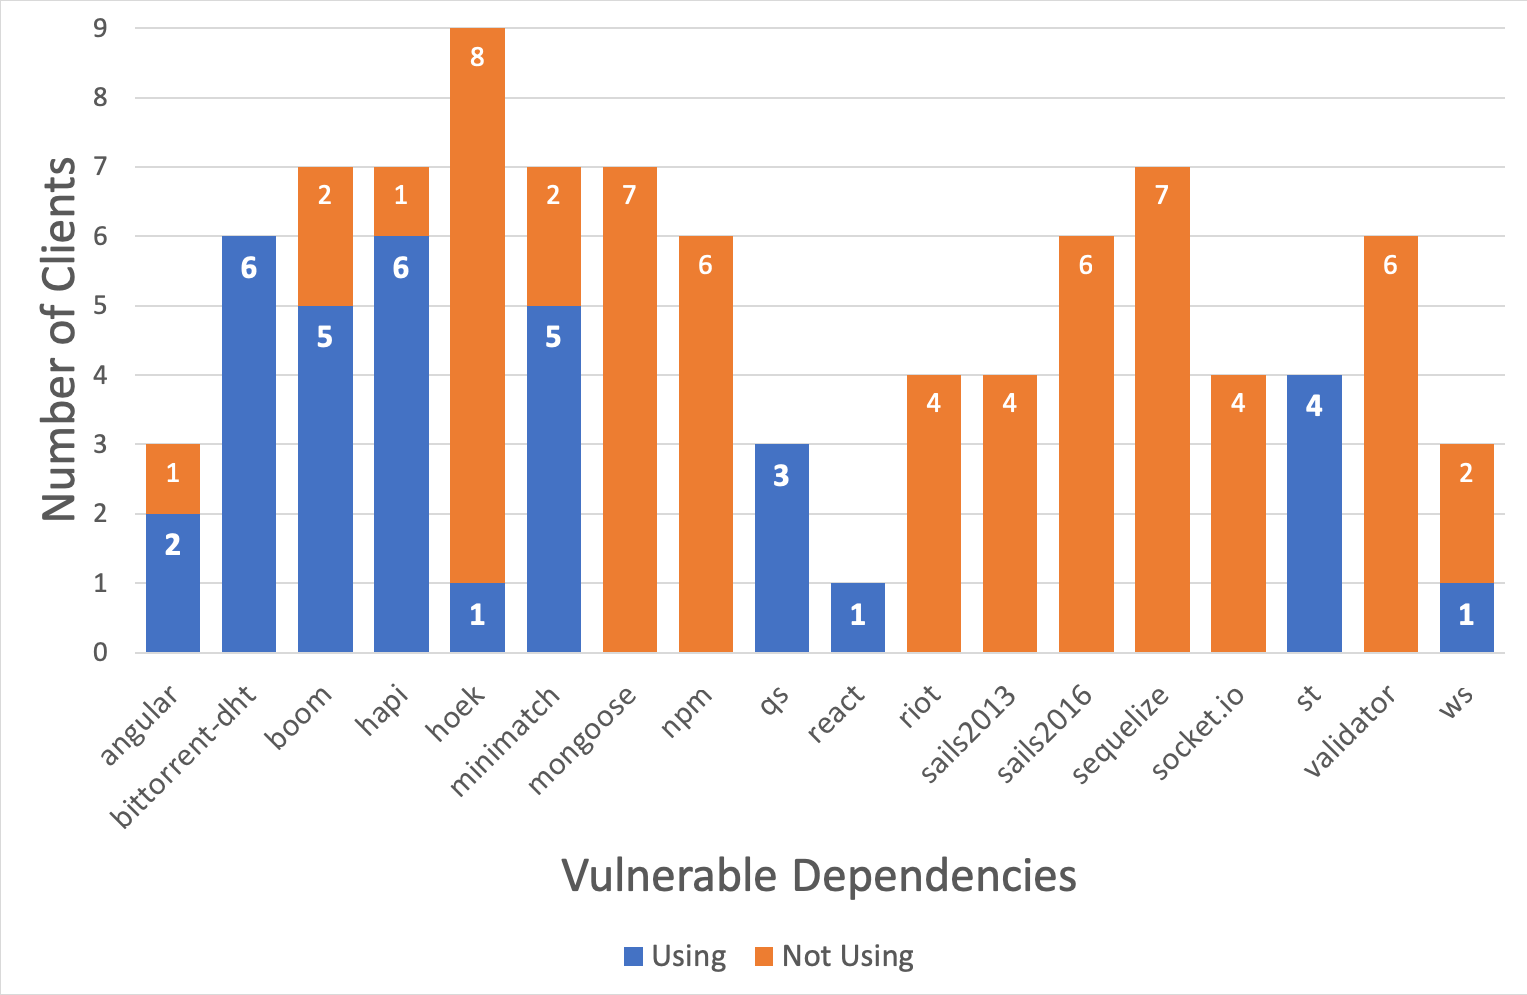
\includegraphics[width=1\textwidth]{images/impact_results.png}
\caption{Proportion of usage of vulnerable functions from third-party libraries}
\label{fig:impactResults}
\end{figure}
%%%%%%%%%%%%%%%%%%%%%%%%%%%%%%%%%%%%%

The results of this study are consistent with the previous studies where I have identified that the assumption of a project been vulnerable because it used a vulnerable function it may be an overestimation.

Detailed information of the client projects as well as the outputs generated by \tool[] to perform this study can be found on the following url: \url{https://github.com/rodrigo-e/ImpactStudy}.

After analyzing the previous results I came with the following implications:
\begin{enumerate}
    \item \textit{Understanding whether or not the vulnerability affects the client code will help developers better plan their library migrations.}
    I speculate that analysis to find whether or not the code is affecting the client code would be beneficial (especially for the novice developer) when making the decision to update. 

    \item \textit{Developers should be encouraged to migrate away from the vulnerable dependency, even if the vulnerable code is not being used.}
    Although there are different reasons for keeping the outdated version (i.e., fix breaks the older version or new changes are not needed), developers should be encouraged to update as soon as the fix is made available.
    Furthermore, I suggest that security only patches should be released.
    This is similar to the Debian ecosystem, where security patches are especially released and not packaged with other updates.
    I believe that this will help towards facilitating smoother library migrations.
\end{enumerate}